\section{Methods}

\subsection{Parameter Generation}
To obtain suitable parameters for the neuromuscular and impedance control
methods we rely on the dueling bandits optimization approach outlined in
\cref{sec:bandit_optimization}. Whereas in \cref{sec:bandit_optimization} we
optimized control parameters to match gait data at different speeds to achieve a
speed-adaptive control, in this work, we optimize control parameters to match
both undisturbed and disturbed gait in order to obtain robust control
parameters. We use the dataset provided by \citet{moore2015elaborate}, which
provides gait data for undisturbed walking and walking with treadmill velocity
disturbances. 

\begin{margintable}    
    \centering
    \normalsize
    \begin{tabular}{ll}
        \multicolumn{2}{l}{Optimized Parameters} \\
        \midrule
        $F_\tn{max}^\tn{ham}$              & $^{F+}G_\tn{ham}^\tn{ham}$   \\
        $F_\tn{max}^\tn{vas}$              & $^{F+}G_\tn{vas}^\tn{vas}$   \\
        $F_\tn{max}^\tn{gas}$              & $^{F+}G_\tn{gas}^\tn{gas}$   \\
        $F_\tn{max}^\tn{sol}$              & $^{F+}G_\tn{sol}^\tn{sol}$   \\
        $F_\tn{max}^\tn{ta}$               & $^{F-}G_\tn{sol}^\tn{ta}$    \\
        $^\tn{off}l_\tn{ta}^\tn{ta}$       & $^{L+}G_\tn{ta}^\tn{ta}$     \\
        $^\tn{off}\phi_\tn{knee}^\tn{vas}$ & ${^\phi}G_\tn{knee}^\tn{vas}$ \\
        $S_0^\tn{vas}$                     & $\epsilon_\tn{SE}^\tn{ap}$   \\
        $S_0^\tn{ham}$                     & $F_\tn{init}^\tn{ham}$       \\
    \end{tabular}
    \caption[Parameters optimized for parameter set generation for experiment
    comparing neuromuscular and impedance control]{Optimized parameters,
    $\Gamma$. We optimize 18 parameters. $F_\tn{max}^m$ refers to muscle $m$'s
    maximum isometric force, $S_0^m$ is muscle $m$'s pre-stimulation,
    $^\tn{signal} G_n^m$ is the gain on a feedback signal from muscle $n$
    acting on muscle $m$, $\epsilon_\tn{SE}^\tn{ap}$ is the tendon reference
    strain of the ankle plantarflexors (sol and gas) and $F_\tn{init}^\tn{ham}$
    is the initial force in the hamstring MTU at
    heelstrike.}\label{tab:nm_params_treadmill_exp}
\end{margintable}
For the neuromuscular control, we use the black-box CMA-ES
optimizer~\citep{hansen2006cma} to obtain parameters that can reproduce the
behavior of each subject in the gait datset. The model proceeds by feeding joint
hip, knee, and ankle angles into the neuromuscular model which generates torques
for the knee and ankle. We optimize the parameters listed in
\cref{tab:nm_params_treadmill_exp} so the model's output torques match those in
the gait dataset. Specifically, we minimize the following cost function:
\begin{align}
    \Gamma &= \argmin_\Gamma \left(\tau_\tn{h} - \tau_\tn{nm} \right)^T
    \left(\tau_\tn{h} - \tau_\tn{nm} \right) + \alpha \xi_\tn{nm}^T \xi_\tn{nm}
\end{align}
where $(\tau_\tn{nm}, \xi_\tn{nm}) = \func{neuro}[\Gamma][]{\theta_\tn{h}}$ are
the torques and muscle activations generated by the neuromuscular model given
the human joint angle trajectories and model parameters $\Gamma$. $\alpha =
0.01$ is a small constant we use to help regularize the solutions and prevent
muscle stimulations from saturating. \Cref{fig:treadmill_nm_fit} shows an
example of the fit achieved to one subject's joint moments.
\begin{figure}[t]
    \centering 
    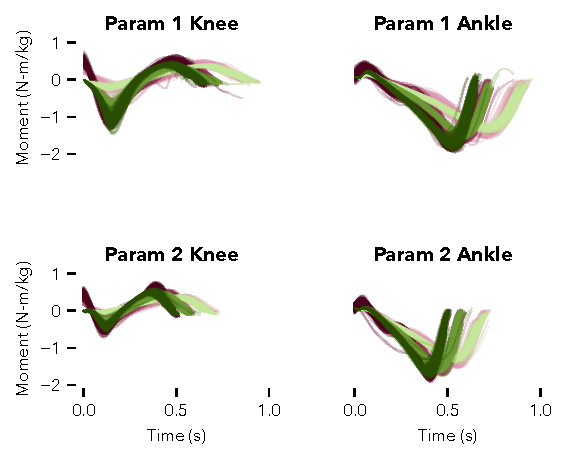
\includegraphics[width=\textwidth]{nm_fit}
    \caption{Example of fit to subject data achieved by neuromuscular model to
    subject 5's data from
    \citet{moore2015elaborate}.}\label{fig:treadmill_nm_fit}
\end{figure}

\todo{fix reference}
To generate parameters for impedance control, which is described in full in
\cref{sec:back_impedance}, we follow a two step procedure: In the first step, we
identify appropriate joint angle thresholds that define the impedance
controller's finite state machine transition rules. The impedance control
transition from phase 1 to phase 2 of stance is based on the knee angle crossing
a threshold. We specify this threshold such that 95\% of steps in the subject's
gait data pass from phase 1 to phase 2. As we use gait data with disturbances,
this procedure automatically sets the threshold such that it allows for a large
degree of gait variation. Next, we identify the ankle angle threshold that
defines the transition between stance phases 2 and 3. Again, we set this
threshold such that 95\% of steps succesfully complete the transition.

Once we identify the joint angle thresholds that define state transitions, we
next fit the impedance parameters within each phase. In each phase, the torque
output of the impedance control is 
\begin{align}
    \tau_\tn{imp} &= -k \left( \theta - \theta_0 \right) - b \dot{\theta} \\
        &= \begin{bmatrix} -\theta & -\dot{\theta} & 1 \end{bmatrix}
            \begin{bmatrix} k \\ b \\ k \theta_0 \end{bmatrix} \\
        &= \Theta \vec{k}
\end{align}
where $\Theta$ is a matrix of the subject's joint angles and velocities and
$\vec{k}$ is a vector of the impedance parameters. Therefore, the squared error
between the subject's joint torque and the impedance control model is
\begin{align}
    \epsilon_\tau & = {\left( \tau_\tn{imp} - \tau_\tn{h} \right)}^T 
        \left( \tau_\tn{imp} - \tau_\tn{h} \right) \\
        &= \vec{k}^T \Theta^T \Theta \vec{k} - 2\tau_\tn{h}^T \Theta \vec{k} 
        + \tau_\tn{h}^T \tau_\tn{h}
\end{align}
To calculate the impedance parameters for each phase we minimize the squared
error subject to the constraints that $k>0$ and ${b > 0}$, which ensures that
the resulting impedance models are stable. Finally, to obtain model parameters
that arerobust to outlier steps in the dataset, we utilize the RANSAC procedure,
which iteratively solves the above optimization on randomly sampled subsets of
the data in order to classify and fit to inliers only
\citep{fischler1981random}.

\begin{figure}[t]
    \centering 
    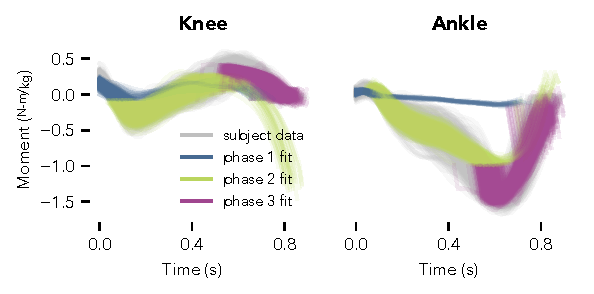
\includegraphics[width=\textwidth]{imp_fit}
    \caption[Example of fit to subject data achieved by impedance control model
    to subject 5's data from \citet{moore2015elaborate}]{Example of fit to
    subject data achieved by impedance control model to subject 5's data from
    \citet{moore2015elaborate}. Note that green trajectories in knee moment plot
    and blue trajectories in ankle moment plot that do not track subject data
    are those that did not successfully transition to the next
    phase.}\label{fig:treadmill_imp_fit}
\end{figure}

\Cref{fig:treadmill_imp_fit} shows an example of the impedance control model
optimized to match one subject's gait data. In this figure, the color of the
lines indicatse the phase of gait. We see that the majority of steps fit the
subject's joint moments (grey) well. However, there are a few steps for which
the color of the line and thus the phase does not transition properly.
Consequently, the resulting torque diverges greatly from the human data. This is
expected as the phase transition angles were selected such that 95\% of steps
pass through each phase transition. We did not allow 100\% percent of steps
through so as to ignore potential outlier steps.

\subsection{Iterative Learning}

\subsection{Experimental Protocol}

We seek to evaluate the robustness of the
